\section{Theoretische Grundlagen}

Um die Fallstudie durchzuführen, wird zunächst der theoretische Rahmen der Arbeit erläutert. In diesem Kapitel wird zunächst der DevOps-Ansatz und Microservices beschrieben. Anschließend wird Containervirtualisierung sowie Kubernetes erklärt.

\subsection{DevOps}

Bevor auf die Architektur und die verwendete Technologien eingegangen wird, ist es wichtig den weiteren Kontext zu betrachten. Wie das Kofferwort "DevOps" bereits andeutet, beschreibt er einen Ansatz für eine effektivere und stärkere Zusammenarbeit zwischen Softwareentwicklung (Development) und IT-Betrieb (Operations). Dabei ist DevOps nicht klar definiert und ist ein Überbegriff für Denkweisen, Kultur, Methoden, Technologien und Werkzeuge. DevOps stellt den Kundennutzen in den Mittelpunkt. Das Ziel ist es ein Unternehmen anpassungsfähiger zu machen und trotzdem   geordnete Prozesse zu wahren. Die Anpassungsfähigkeit wird hier häufig mit der Time to Market gemessen. Diese Kennzahl sagt aus wie lange es dauert eine Änderung auf die Produktionsumgebung zu bringen.

\begin{figure}[H] 
    \centering
    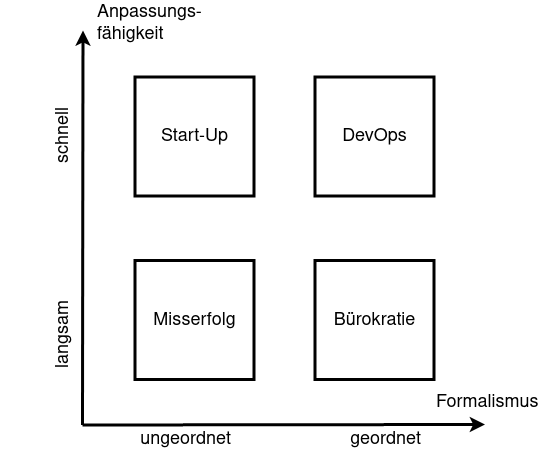
\includegraphics[width=0.7\textwidth]{figures/DevOpsDiagramm.png}
    \caption{Kategorisierung von Unternehmen}
\end{figure}

Um DevOps in Unternehmen umzusetzen reicht es nicht die entsprechenden Werkzeuge einzuführen, sondern es muss zu einem Kulturwandel kommen.

DevOps ist eine Sammlung an Methoden und Denkweisen, welche sich immer weiter verbreiten. Das Vorgehen in der Fallstudie dieser Arbeit kommen auch DevOps-Werkzeuge zum Einsatz. Da die gewählten Technologien und Architekturmuster sich nicht nur auf den Entwurf sondern auch


Eine der wichtigsten Werkzeuge von DevOps ist Continuous Delivery.

\subsection{Microservices}

Im Mittelpunkt dieser Arbeit stehen Microservices. Bei Microservices handelt es sich um ein Architekturmuster zur Modularisierung von Software (\cite[S. 15]{newmanMicroservices2015}). Obwohl der Begriff Microservices noch realtiv jung ist, sind die dahinterstehenden Konzepte bereits älter (\cite[S. 15]{newmanMicroservices2015}). Zur Verständlichkeit und leichteren Weiterentwicklung werden große Systeme werden schon lange in kleine Module unterteilt. Die Besonderheit von Microservices liegt darin, dass die Module einzelne Programme sind. Ein solches einzelnes Programme wird als Microservice bezeichnet. \\
\\
Microservices sind ein Architekturmuster. Architekturmuster beschreiben die Grundstruktur von Systemen in der Softwareentwicklung. Microserices werden als Architekturmuster in die Kategorie der verteilten Systeme eingeordnet. Die einzelnen Microservices laufen zumeist auf vielen unterschiedlichen Rechnern. Die Microservices sind dabei voneinander unabhängig und kommunizieren in einem Netzwerk über festgelegte Schnittstellen miteinander. \\
\\
Microservices sind also das Gegenteil von klassischen monolithischen Softwarearchitekturen. Monolithische Software ist eine einzelne, zusammenhängende und untrennbare Einheit. Dies macht die Erweiterbarkeit und Warbarkeit deutlich schwieriger, da Teile des Systems nur mit erheblichem Aufwand angepasst werden können. Es kann zu nicht vorhersehbaren Abhängigkeiten kommen. Die Wiederverwendbarkeit von Teilen der Software gestaltet sich aufwendiger. Lastverteilung und Skalierung ist problematisch. Durch Modualisierung lassen sich viele dieser Nachteile abschwächen, können jedoch nicht komplett ausgemerzt werden. Um diese Nachteile zu umgehen sind Microservices entstanden. Doch neben vielen Vorteilen kommen Microservices auch mit Herausforderungen. Im nachfolgenden Abschnitt werden die genauen Vor- und Nachteile genauer erläutert. \\
\begin{figure}[H] 
    \centering
    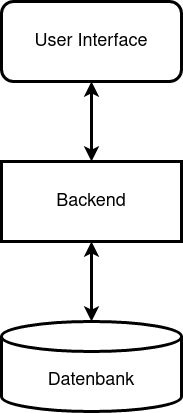
\includegraphics[width=0.2\textwidth]{figures/Monolith.png}
    \caption{Aufbau einer monolithischen Architektur}
\end{figure}
\begin{figure}[H] 
    \centering
    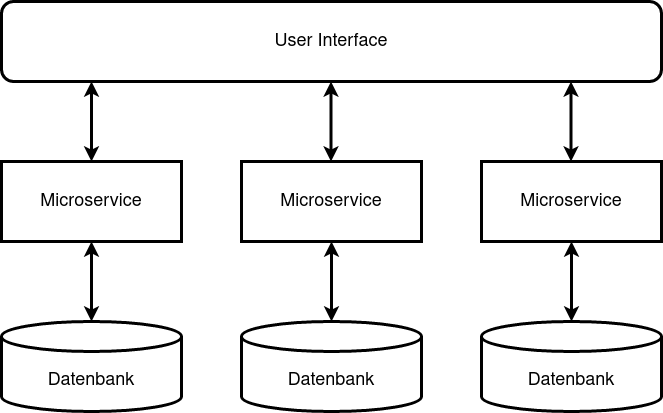
\includegraphics[width=0.71\textwidth]{figures/Microservices.png}
    \caption{Aufbau einer Microservice-Architektur}
\end{figure}

Der Begriff Microservice ist nicht fest definiert (\cite[S. 2]{wolffMicroservices2018}), deshalb werden im nachfolgenden Kapitel die wichtigsten Eigenschaften und Merkmale betrachtet.
\\
Dabei werden Microservices häufig im geschäftlichen Umfeld eingesetzt (\cite[S. 15]{newmanMicroservices2015}). \\
\\
Microservices sollen nur eine Aufgabe erledigen, diese jedoch bestmöglich. Dieser Ansatz ist nicht neu und entstammt der UNIX-Philosophie: "Mache nur eine Sache und mache sie gut" (Douglas McIlroy).
Wie der Name "Microservices" bereits andeutet, handelt es sich dabei offensichtlich um kleine Services. Eine genaue Festlegung wie groß die Services sein sollten gibt es jedoch nicht. Die Anzahl der Codezeilen (Lines of Code) können einen Hinweis geben, jedoch sind derartige Kriterien stark von der Programmiersprache und dem verwendeten Technologie-Stack abhängig. Stattdessen sollte sich die Größe an fachliche Gegebenheiten anpassen. Je kleiner die Services gestaltet werden, umso stärker kommen die in den nachfolgenden Abschnitten beschriebenen Vor- und Nachteile zur Geltung. Des Weiteren sollte ein Microservice nur so Groß sein, dass er von einem einzigen Entwicklerteam betreut werden kann. Die Größe eines Microservices ist für die Definition also nicht zwangsläufig entscheidend (\cite[S. 2]{wolffMicroservices2018}). \\
\\
Der Name "Microservices" deutet schon an, dass es sich offensichtlich um kleine Services handelt.
Eine objektive Messung der Größe ist jedoch nicht möglich. Um die Größe eines Microservices zu bestimmen, könnte man beispielsweise die Anzahl der Codezeilen (LoC) verwenden. Doch die Lines of Code hängen starkt von der verwendeten Programmiersprache und dem Technologie-Stack ab. Eine Messung der Größe nach rein objektiven Kriterien macht demnach keinen Sinn (\cite[S. 31]{wolffMicroservices2018})(\cite[S. 22]{newmanMicroservices2015}). Stattdessen sollte sich die Größe an die fachlichen Gegebenheiten richten. Je kleiner die Services werden desto mehr kommen die in den nächsten Abschnitten beschriebenen Vor- und Nachteile zur Geltung. Ein Microservice sollte von einem einzigen Enticklerteam gehandhabt werden (\cite[S. 23]{newmanMicroservices2015}). Falls das nicht mehr möglich ist, könnte es darauf hindeuten, dass der Microservice zu groß ist. \\
\\
Die Teamgröße beschrenkt die Größe eines Microservices, um die Unabhängigkeit der Entwicklerteams zu gewährleisten. Ein einzelner Entwickler sollte in der Lage sein den kompletten Microservice zu verstehen. Die Infrastruktur begrenzt auch die Größe. Ist die Bereitstellung eines Services sehr aufwendig, sollte die Anzahl der Microservices eher geringer sein. Auch die Kommunikation zwischen den Services und somit die Netzwerkauslastung nimmt mit der Anzahl zu. Das ist ebenfalls ein Grund für nicht zu kleine Services.
\\
Microservices laufen als eigenständige Programme und müssen unabhängig voneinander deploybar sein. Jeder Microservice ist ein eigener Prozess, welcher isoliert von den anderen abläuft. Die Isolierung trägt dazu bei, dass verteilte System besser zu verstehen aber auch keine unbemerkten Abhängigkeiten zwischen den Services entstehen zu lassen. Neue Technologien wie Containervirtualisierung können dies erleichtern. Die Kommunikation der Services erfolgt über ein Netzwerk und mittels sprachunabhängiger Schnittstellen (API). \\
\\
Ein Microservice bildet eine eigenständige und klar definierte Funktion einer Applikation ab. Der Zugriff auf den Service erfolgt ausschließlich über eine klar definierte Schnittstelle (\cite[S. 64]{trempArchitekturen2021}). Wo genau die Aufteilung in Microservices vorgenohmen werden kann wird in einem späteren Kapitel genauer diskutiert. Es ist jedoch durchaus eine komplexe und schwierige Aufgabe.
\\
Eine ausreichende Eigenständigkeit ist nur gegeben, sobald die Services unabhängig voneinander verändert und bereitgestellt werden können. Ein Entwicklerteam sollte sich bei der Implementierung von Änderungen oder neuen Funktionen nicht mit anderen Teams absprechen müssen. \\
\\
Das Gesetz von Conaway von Melvin Edward Conway besagt, dass "Organisationen die Systeme entwerfen sind gewzungen Entwürfe zu erstellen die die Kommunikationsstrukturen dieser Organsiationen abbilden." Vereinfacht gesagt, wenn zwei Entwicklerteams in einem Unternehmen ein neues Softwaresystem entwickeln, dann wird mit großer Wahrscheinlichkeit das neue Softwaresystem unabhängig von den fachlichen Anforderungen auch aus zwei großen Komponenten bestehen. Die Schnittstellen zwischen diesen zwei Komponenten werden eine ähnliche Qualität wie die zwischenmenschlichen Kommunikation zwischen den beiden Entwicklerteams haben. Studien der Havard Business School belegen, dass diese These in der Realität meistens zutreffend ist.  \\
\\
Das CAP-Theorem kann auf alle verteilte Systeme und somit auch auf Microservices angewendet werden. Es besagt, dass es niemals möglich ist, gleichtzeitig die drei Eigenschaften Konsistenz (Consistency), Availability (Verfügbarkeit) und Ausfalltoleranz (Partition Tolerance) zu gewährleisten.

\subsubsection{Serviceorientierte Architekturen}

An dieser Stelle muss ein kurzer Exkurs zu serviceorientierten Architekturen (SOA) gemacht werden, da der Begriff häufig im Zusammenhang genannt wird. 

Serviceorientierte Architektur ist ein Designansatz (\cite[S. 29]{newmanMicroservices2015}). Wie der Name schon andeutet ist das Prinzip sehr ähnlich zu Microservices. Auch bei SOA gibt es Services, welche über das Netzwerk miteinander kommunizieren.
  
Es gibt durchaus Definitionen welche Microservice und SOA als identisch ansehen. 

Services bei SOA werden jedoch nicht neu entwickelt. Die Funktionalität ist in den betrieblichen Anwendungen bereits vorhanden. Durch einen SOA-Ansatz sollen diese Funktionalitäten durch Services von außerhalb der Anwendung zugreifbar gemacht werden. Das Ziel ist es eine flexiblere Gesamtstruktur der IT in einem Unternehmen zu haben und Services wiederverwenden zu können. Es bedeutet jedoch nicht zwanglsäufig das große monolithische Anwendungen in kleine Services aufgeteilt werden. Eine große Anwendung kann auch aus mehreren Service-Komponenten besitzen, die dessen Dienste für andere Anwendungen verfügbar machen, ohne den eigentlichen Monolithen aufzuteilen. Über die Service sollen Geschäftsprozesse abgebildet werden (\cite[S. 2]{wolffMicroservices2018}).

Der größte Unterschied liegt jedoch auf der Ebene an der beide Ansätze ansetzen. Bei Microservices handelt es sich wie bereits erklärt um Architekturmuster, also einen konkreten Ansatz wie eine Anwendung entworfen werden kann. SOA setzt bei der gesamten IT eines Unternehmens an. SOA beschreibt wie viele Systeme in einem Unternehmen miteinander interargieren. Microservices beschreiben die Architektur von einem einzigen System. 


\subsubsection{Vorteile}

Das Aufteilen von Software bringt wichtige Vorteile mit sich.

\paragraph{Modularisierung}
Bei klassischen Software-Monolithen, welche aus Komponenten zusammengestellt wird, entstehen schnell unerwünschte Abhängigkeiten. Die viele Abhängigkeiten erschweren die Wartung oder Weiterentwicklung. Da die einzelnen Microservices eigene Programme sind, herrscht eine starke Modularisierung. Die Programme sind eigenständig und kommunizieren nur über explizite Schnittstellen. Ungewollte Abhängigkeiten entstehen hier deutlich schwerer. (\cite[S. 3]{wolffMicroservices2018})

In der Praxis wird die Architektur von Deployment-Monolithen meistens zunehmend schlechter. (\cite[S. 3]{wolffMicroservices2018})

\paragraph{Austauschbarkeit}
Da Microservices nur über eine explizite Schnittstelle genutzt werden, können sie einfach durch einen Service, der die selbe Schnittstelle anbietet ersetzt werden. Bei der Ersetzung ist der neue Service nicht an den Technologie-Stack des alten Service gebunden. Auch die Risiken werden geringer, da bei schwerwiegenden Fehlentscheidungen in der Entwicklung, ein Austausch mit weniger Aufwand verbunden ist. (\cite[S. 4]{wolffMicroservices2018})

Sie können auch deutlich schneller eingesetzt werden. (Time to Market)

Das gesamte neu schreiben eines Microservices ist in der Regel nicht besonders schwer. Viele Unternehmen scheitern an der Wartung oder Erweiterungen von alten monolithischen Systemen (\cite[S. 29]{newmanMicroservices2015}). Da Problem ist das die Ablösung dieser großen Systeme eine fast unmöglichen Mammutaufgabe ist.

\paragraph{Skalierbarkeit}
Durch die Unabhängigkeit der Microservices können sie auch unabhängig voneinander skaliert werden. So kann eine einzelne Funktionalität, welche stärker genutzt wird, skaliert werden, ohne das gesamte System zu skalieren. (\cite[S. 5]{wolffMicroservices2018})

Dadurch können gezielt Falschenhälse in der Anwendung entsprechend hochskaliert werden.

Beim Einsatz von Cloudanbietern wie AWS ist es möglich eine Skalierung nach dem genauen Bedarf vorzunehmen. So wird nur die tatsächlich Gebrauchte Leistung des Systems bezahlt. Aber auch bei on-Premise Lösungen profitiert man von einer effektiveren Lastausnutzung. Auch die Verteilung der Last ist einfacher, da die Services auf unterschiedlichen Maschinen laufen. 

Es gibt wenige Architekturmuster wie dieses, welche so eng mit Kosteneinsparungen verbunden sind. (\cite[S. 27]{newmanMicroservices2015}).

\paragraph{Technologiefreiheit}

Des Weiteren führt die Unabhängigkeit auch zu einer großen Technologiefreiheit. Die verwendeten Technologien müssen schließlich nur in der Lage sein die explizite Schnittstelle anzubieten. (\cite[S. 5]{wolffMicroservices2018})

Statt auf einen Technologie-Stack als Kompormiss zu verwenden, kann für jeden Service die am besten geeigneten Technologien ausgewählt werden. 

Außerdem können neue Technologien auch leichter angewendet werden. Bei einer großen monolithischen Anwendung ist eine Umstellung auf beispielsweise ein neue Programmiersprache ein schwieriger und langwieriger Prozess. Bei Microservices kann die neue Sprache zuerst an einem einzelnen Service getestet werden und dann schrittweise das ganze System umgestellt werden. Oder eben nur die Services für welche die neue Sprache auch wirklich Vorteile besitzt. (\cite[S. 25]{newmanMicroservices2015}).

Ein Nebeneffekt von dieser Technologiefreiheit ist auch, dass die Auswirkungen von falschen Entscheidungen über die Einführung von neuen Technologien deutlich reduziert. 


\paragraph{Continuous Delivery}

Ein wesentlicher Grund für die Einführung ist Continuous Delivery. Die kleinen Microservices können leichter deployt werden und das Deployment bietet weniger Gefahren und ist einfacher abzusichern, als bei einem Monolithen. (\cite[S. 5]{wolffMicroservices2018}) \\
\\
Das schnelle und größtenteils automatisierte Ausliefern von Software ist wichtig. In der der schnelllebigen Zeit ist man nur im Vorteil wenn neue Features und Fehlerbehebungen so schnell wie ihren Weg zum Benutzer finden. Microservices können schneller und leichter deployt werden als große Monolithen. Vor allem bei geringen Änderungen von einigen Codezeilen ist der gesamte Deployment Prozess von Monolithen sehr nervig.

Durch Ihre Unabhängigkeit können nur einzelne Services nach Änderungen neu bereitgestellt werden. Auch hier ist sind die Auswirkungen von Fehlern geringer. Ist eine Auslieferung fehlerhaft ist nicht das ganze System davon betroffen, sondern lediglich ein Service. Auch kann bei Microservices leicht noch eine alte Version desselben Services betrieben werden, bis die fehlerfreie Funktion der neuen Version gewährleistet ist. Bei einem Monolithen wäre der Ressourcenverbrauch in so einem Fall doppelt so hoch, wie die eigentliche Anwendung benötigt. \\

\subsubsection{Herausforderungen}

Doch natürlich haben Microservices wie jedes Architekturmuster auch einige Nachteile.

\paragraph{Versteckte Beziehungen}

\paragraph{Refactoring}

\paragraph{Fachliche Architektur}

\paragraph{Komplexität}

\paragraph{Verteilte Systeme}

\subsubsection{Architektur}

Die Architektur bei Micrservices ist das Finden von Kompromissen. Die einzelnen Entwicklerteams sollten viel Freiheit haben, um die nach ihrer Meinung am Besten geeigneten Technologien für ihren Service zu verwenden. Es macht jedoch Sinn gewisse Vorgaben und Rahmenbedingungen vorzugeben. Die Beschränkung auf eine Auswahl von beispielsweise fünf Programmiersprachen macht Sinn, um Wissen nicht zu weit zu verstreuen. Für die Schnittstellen ist es sinnvoll einige wenige Schnittstellenarten festzulegen, die von allen Services verwendet wird.  \\
\\
Die Mikroarchitektur, also die Architektur mit der ein einzelner Service implementiert wurde, sollte von außen nicht sichtbar sein und besitzt somit für das Gesamtsystem keine Relevanz. \\
\\
Die fachliche Archtiektur, also die Aufteilung in verschiedene Bereiche, die jeweils von einem Microservice umgesetzt werden. Wo bei dieser Aufteilung die Grenzen gezogen werden ist eine der zentralen Herausforderungen (\cite[S. 102]{wolffMicroservices2018}). Das entscheidende Kriterium für die Aufteilung ist, dass Änderungen möglichst nur einen Service betreffen und somit von nur einem Team durchgeführt werden können. Dadurch ist wenig Abstimmung zwischen den Entwicklerteams notwendig und die Vorteile der Microservices kommen erst richtig zur geltung. Jeder Microservice solle also eine fachlichen Kontext darstellen, der eine abgeschlossene Funktionalität darstellt. \\
\\
Natürlich sind die Microservices nie vollständig voneinander unabhängig. Es wird Services geben die, die Funktionalität anderer Services aufrufen. Zu viele solcher Verbindungen führen jedoch zu einer hohen Abhängigkeit und widersprechen dem Microservice-Ansatz. Eine lose Kopplung, also nur wenige Abhängigkeiten sind erstrebenswert, da so sich Änderungen so nur auf einen Service auswirken. Benötigt ein Microservice viele Funktionalitäten von einem anderen Microservice kann das ein Hinweis auf eine schlechte Aufteilung sein und die Services sollten an einer anderen Stelle aufgeteilt werden oder womöglich direkt zusammen gelegt werden. Innerhalb eines Micrservice sollten die Komponenten und Module des Programms jedoch eine starke Kopplung besitzen. Dadurch wird gewährleistet, dass die Bestandteile wirklich zusammengehören. \\
\\
Zyklische Abhängigkeiten sind auch zu vermeiden, da dort ohne weitere Abstimmung Änderungen in einem der beiden Services nicht möglich sind. \\
\\
Eine bewährter Ansatz für den Anfang der Architektur ist es, mit großen Service zu beginnen und diese aufzuteilen. Einen großen Service aufzuteilen ist einfach. Die Gesamtarchitektur von vielen kleinen Services zu überarbeiten jedoch sehr komplex. \\

Herausforderung: Microservice-Systeme sind schwer änderbar (auf Makro Ebene)

Architektur eines Microservice: Erklärung Schichtenarchitektur, wenige Vorgaben, wird vom Team gehandhabt

\subsubsection{Integration und Kommunikation}

Microservices müssen miteinander kommunizieren. Die Integration der Services ist auf drei verschiedenen Ebenen denkbar.

\paragraph{UI}

\paragraph{Datenbank}

\paragraph{Microservices}

Zuletzt müssen natürlich auch Microservices direkt miteinander kommunizieren, um so Funktionalität von anderen Services aufzurufen. Die meist verbreitetste Technologie ist HTTP REST. Es gibt auch weitere Ansätze wie SOAP oder Message-Systeme.

{Definition REST}


\subsubsection{Bereitstellung und Betrieb}

\subsubsection{Fazit}

Viele Vorteile
Wichtige Dinge um die sich gekümmert werden müssen: Skalierung, Deployment, Service Discovery werden durch Kubernetes übernommen und erleichtert.


\subsection{Containervirtualisierung}

Früher wurden Anwendungen auf physischen Rechnern ausgeführt. Wenn mehrere Anwendungen auf einem Rechner liefen, konnte eine Anwendung Ressourcen wie die Rechenleistung der anderen Anwendung wegnehmen. Durch Virtualisierung von Hardware konnte das Problem gelöst werden, indem mehrere virtuelle Maschinen auf einem physischen Rechner betrieben werden. Virtuelle Maschinen besitzen dieselben Funktionen wie ein physischer Rechner und führen ein eigenes Betriebssystem aus. Dadurch ist diese Art der Virtualisierung nicht leichtgewichtig. Bei der Containervirtualisierung werden nur die Ressourcen des Betriebssystems des Betriebssystems zur Verfügung gestellt, welche auch wirklich benötigt werden. Containervirtualisierung ist deshalb leichtgewichtig.

Ein weiteres Problem ist, wie Microservices aber auch andere verteilte Systeme über große Netzwerke mit vielen verschiedenartigen Rechnern bereitgestellt werden können. Es wurde also eine zuverlässige Methode gesucht wie Software auf diversen Rechnern immer gleich läuft. Auch dieses Problem schafft Containervirtualisierung aus dem Weg, indem es Software mit allen Abhängigkeiten, Bibliotheken, Compilern und Konfigurationen in eine standardisierte und einheitliche Komponente verpackt: Der Container. 
Ein Image einer virtuellen Maschine besitzt auch alle diese Eigenschaften, enthält aber noch viel mehr als wie die Anwendung wirklich für die Ausführung benötigt.

Vorteile zu VMs:
- Container laufen auf der realen CPU, somit kein zusätzlicher Aufwand für Virtualisierung
- Container enthält nur die Dateien, die wirklich benötigt werden, daher viel kleiner
- Dateisystem-Layern, könen von mehreren Container genutzt und wiederverwendet werden, effiziente Platznutzung

Eigenschaften von Images:
- Wiederverwendbar
- Kann überall laufen wo die entsprechende Container-Engine läuft und ausreichend Ressourcen vorhanden sind
- Läuft überall gleich (Container-Format muss unterstützt werden)
- Keine Abhängigkeit von unterschiedlichen Distributionen, Bibliotheken und Software-Versionen auf dem Rechner (lediglich abhängig von Betriebssystem-Kernel)

Ein weiteres Problem was letztendlich zur Containervirtualisierung führte, ist die Frage wie verteilte Systeme (microservices) über große Netzwerke mit verschiedenartigen Rechnern bereitgestellt werden können. 

Container revolutionieren also die Bereitstellung von Anwendungen, haben jedoch auch eine große Auswirkung auf die Anwendungsarchitektur und entfalten so beispielsweise das volle Potential von Microservices.
In der steigenden Beliebtheit von Microservice-basierten Anwendungen bestehend aus Container sehen manche eine ähnliche Revolution wie die in den 1990er-Jahren objektorientierte Programmierung. (\cite[S. 1]{burnsDesign2016})

{Vorteile}

Container eignen sich aufgrund dieser Eigenschaften perfekt, Microservice-basierte Anwendungen zusammenzustellen und auszuführen. 

Container sind normalerweise unveränderlich. Soll ein Container geändert werden, so wird der alte Container gegen einen neuen ausgetauscht.

Ein Container besitzt sein eigenes Dateisystem, Anteil an CPU, Speicher und Prozessraum. 

Containervirtualisierung 

\subsection{Kubernetes}

Der Name Kubernetes ist Griechisch und bedeutet Steuermann. Kubernetes wird häufig auch mit dem Kürzel "K8s" abgekürzt. Kubernetes ist jedoch kein Betriebssystem. Es benötigt ein installiertes Betriebssystem auf den Nodes.

Kubernetes ist eine Open-Source-Plattform zur Orchestrierung und Verwaltung von Container-Awendungen. Wie Kubernetes bei der Bereitstellung und dem Betrieb von Microservices hilft wird in diesem Abschnitt erklärt. Zuerst muss jedoch Containervirtualisierung verstanden werden.

Kubernetes bietet viele Funktionen, die helfen eine entkoppelte Microservice-Architektur zu bauen.

\subsubsection{Aufbau}



\subsubsection{Objekte}

\subsubsection{Wobei hilft Kubernetes im Bezug auf Microservices}

- Service Discovery
- Load Balancing
- Skalierbarkeit
- Monitoring (evtl. auch Logging)
- Deployment

\subsubsection{Kubectl}

\subsubsection{Minikube}

Minikube ist ein Werkzeug, um ein lokales Kubernetes Cluster zu betreiben. Minikube erstellt ein Cluster bestehend aus nur einem Node in einer virtuellen Maschine. Der Node fungiert dabei sowohl als Master sowie auch als Worker. Minikube unterstützt mittlerweile auch den Betrieb mit mehreren Nodes. Des Weiteren kann das Cluster auch in einem Docker Container anstatt in einer virtuellen Maschine betrieben werden. Da Minikube über eine virtuelle Maschine oder in einem Docker Container läuft, kann minikube auch über Linux hinaus auf Windows oder MacOS betrieben werden.
